\documentclass[margin={0 0 3pt 0}]{standalone}
\usepackage{tikz,xcolor-material}
\begin{document}
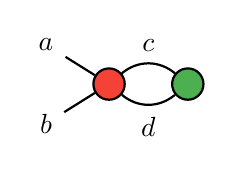
\begin{tikzpicture}[inner sep=4pt, thick, baseline=-0.1cm]
  \path node (M)  at (0,0) [circle, draw, fill=MaterialRed] {}
        node (v)  at (1,0) [circle, draw, fill=MaterialGreen] {}
        node (Ma) at (-0.8, 0.5) {$a$}
        node (Mb) at (-0.8,-0.5) {$b$};
  \draw (M) to [bend left=40,  above] node {$c$} (v)
        (M) to [bend right=40, below] node {$d$} (v)
        (M) -- (Ma)
        (M) -- (Mb);
\end{tikzpicture}
~$=\lambda$%
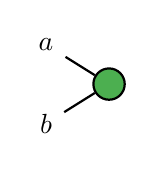
\begin{tikzpicture}[inner sep=4pt, thick, baseline=-0.1cm]
  \path node (v)  at (0,0) [circle, draw, fill=MaterialGreen] {}
        node (va) at (-0.8, 0.5) {$a$}
        node (vb) at (-0.8,-0.5) {$b$};
  \draw (v) -- (va) (v) -- (vb);
\end{tikzpicture}
\end{document}
